\section{耗散粒子动力学}
%%%%%%%%%%%%%%%%%%%%%%%%%%%%%%%%%%%%%%%%%%%%%%%%%%%%%%%%%%%%%%%%%%%%%%%%%%
\subsection{简介}
\frame{ \frametitle{耗散粒子动力学简介}
  \begin{itemize}
  \item 耗散粒子动力学(DPD)是一种适合模拟简单和复杂流体动力学和流变性能的介观
        尺度方法.
  \item 由Hoogerbrugge与Koelman首先提出, 旨在解决经典分子动力学难以解决的流体
        时间和空间尺度问题.
  \item 应用: 各类复杂的流体流动, 如相分离, 蛋白质等大分子悬浮, 表面活性剂, 胶
        体输运, 稀释聚合物溶液, 生物薄膜, 以及介观尺度的多相流动现象.
  \end{itemize}
}
%%%%%%%%%%%%%%%%%%%%%%%%%%%%%%%%%%%%%%%%%%%%%%%%%%%%%%%%%%%%%%%%%%%%%%%%%%
\subsection{基本思想}
\frame{\frametitle{运动方程}
\begin{itemize}
\item 牛顿运动方程描述DPD粒子运动
  \[
  \frac{d\mathbf{r}_i}{dt} = \mathbf{v}_i,   
  \frac{d\mathbf{v}_i}{dt} = \mathbf{f}_i = \mathbf{f}_i^{\text{int}} + \mathbf{f}_i^{\text{ext}}
  \]
 
\item DPD粒子间作用力包括保守力, 耗散力及随机力:
  \[
  \mathbf{F}_{ij}^C = a_{ij}w^C(r_{ij})\mathbf{\hat{r}}_{ij}
  \]
  \[
  \mathbf{F}_{ij}^D = -\gamma w^D(r_{ij})\Big(\mathbf{\hat{r}}_{ij}\cdot \mathbf{v}_{ij}\Big)\mathbf{\hat{r}}_{ij}
  \]
  \[
  \mathbf{F}_{ij}^R = \sigma w^R(r_{ij})\xi_{ij}\mathbf{\hat{r}}_{ij}
  \]
保守力权函数$w^C(r_{ij})$, 一般取为$1-r_{ij}$.
\end{itemize}
}
%%%%%%%%%%%%%%%%%%%%%%%%%%%%%%%%%%%%%%%%%%%%%%%%%%%%%%%%%%%%%%%%%%%%%%%%%%

\frame{\frametitle{热力学平衡条件}
\begin{itemize}
\item 为了维持系统温度不变, 根据随机耗散理论及能量守恒定律, 耗散力与
随机力系数, 以及耗散力权函数和随机力权函数必须满足以下关系

\[
\sigma^2=2\gamma k_BT
\]
\[
w^D(r_{ij})=\Big[w^R(r_{ij})\Big]^2
\]

耗散力权函数$w^D(r_{ij})$一般取$(1-r_{ij})^2$
\end{itemize}
}

%%%%%%%%%%%%%%%%%%%%%%%%%%%%%%%%%%%%%%%%%%%%%%%%%%%%%%%%%%%%%%%%%%%%%%%%%%
\subsection{简单的算例}
\frame{\frametitle{简单流体的模拟}
\begin{center}
  \animategraphics[width=0.9\textwidth, autoplay, loop]{5}{./animate/Poise/}{1}{20}
\end{center}
}

\frame{\frametitle{高分子链在微直通道中的运动}
\begin{center}
\animategraphics[width=0.9\textwidth, autoplay, loop]{5}{./animate/Chain=/}{1}{30}
\end{center}
}
\frame{\frametitle{高分子链在微缩通道中的运动}
\begin{center}
  \animategraphics[width=0.9\textwidth, autoplay, loop]{5}{./animate/ChainT/}{1}{30}
\end{center}
}

\frame{\frametitle{高分子链在微缩通道中的运动}
\begin{center}
  \animategraphics[width=0.9\textwidth, autoplay, loop]{5}{./animate/ChainY/}{1}{30}
\end{center}
}

\section{细胞力学模型}
\subsection{细胞吸入实验简介}
\frame{\frametitle{细胞吸入实验简介}
  \begin{columns}
  \begin{column}[b]{0.52\textwidth}
 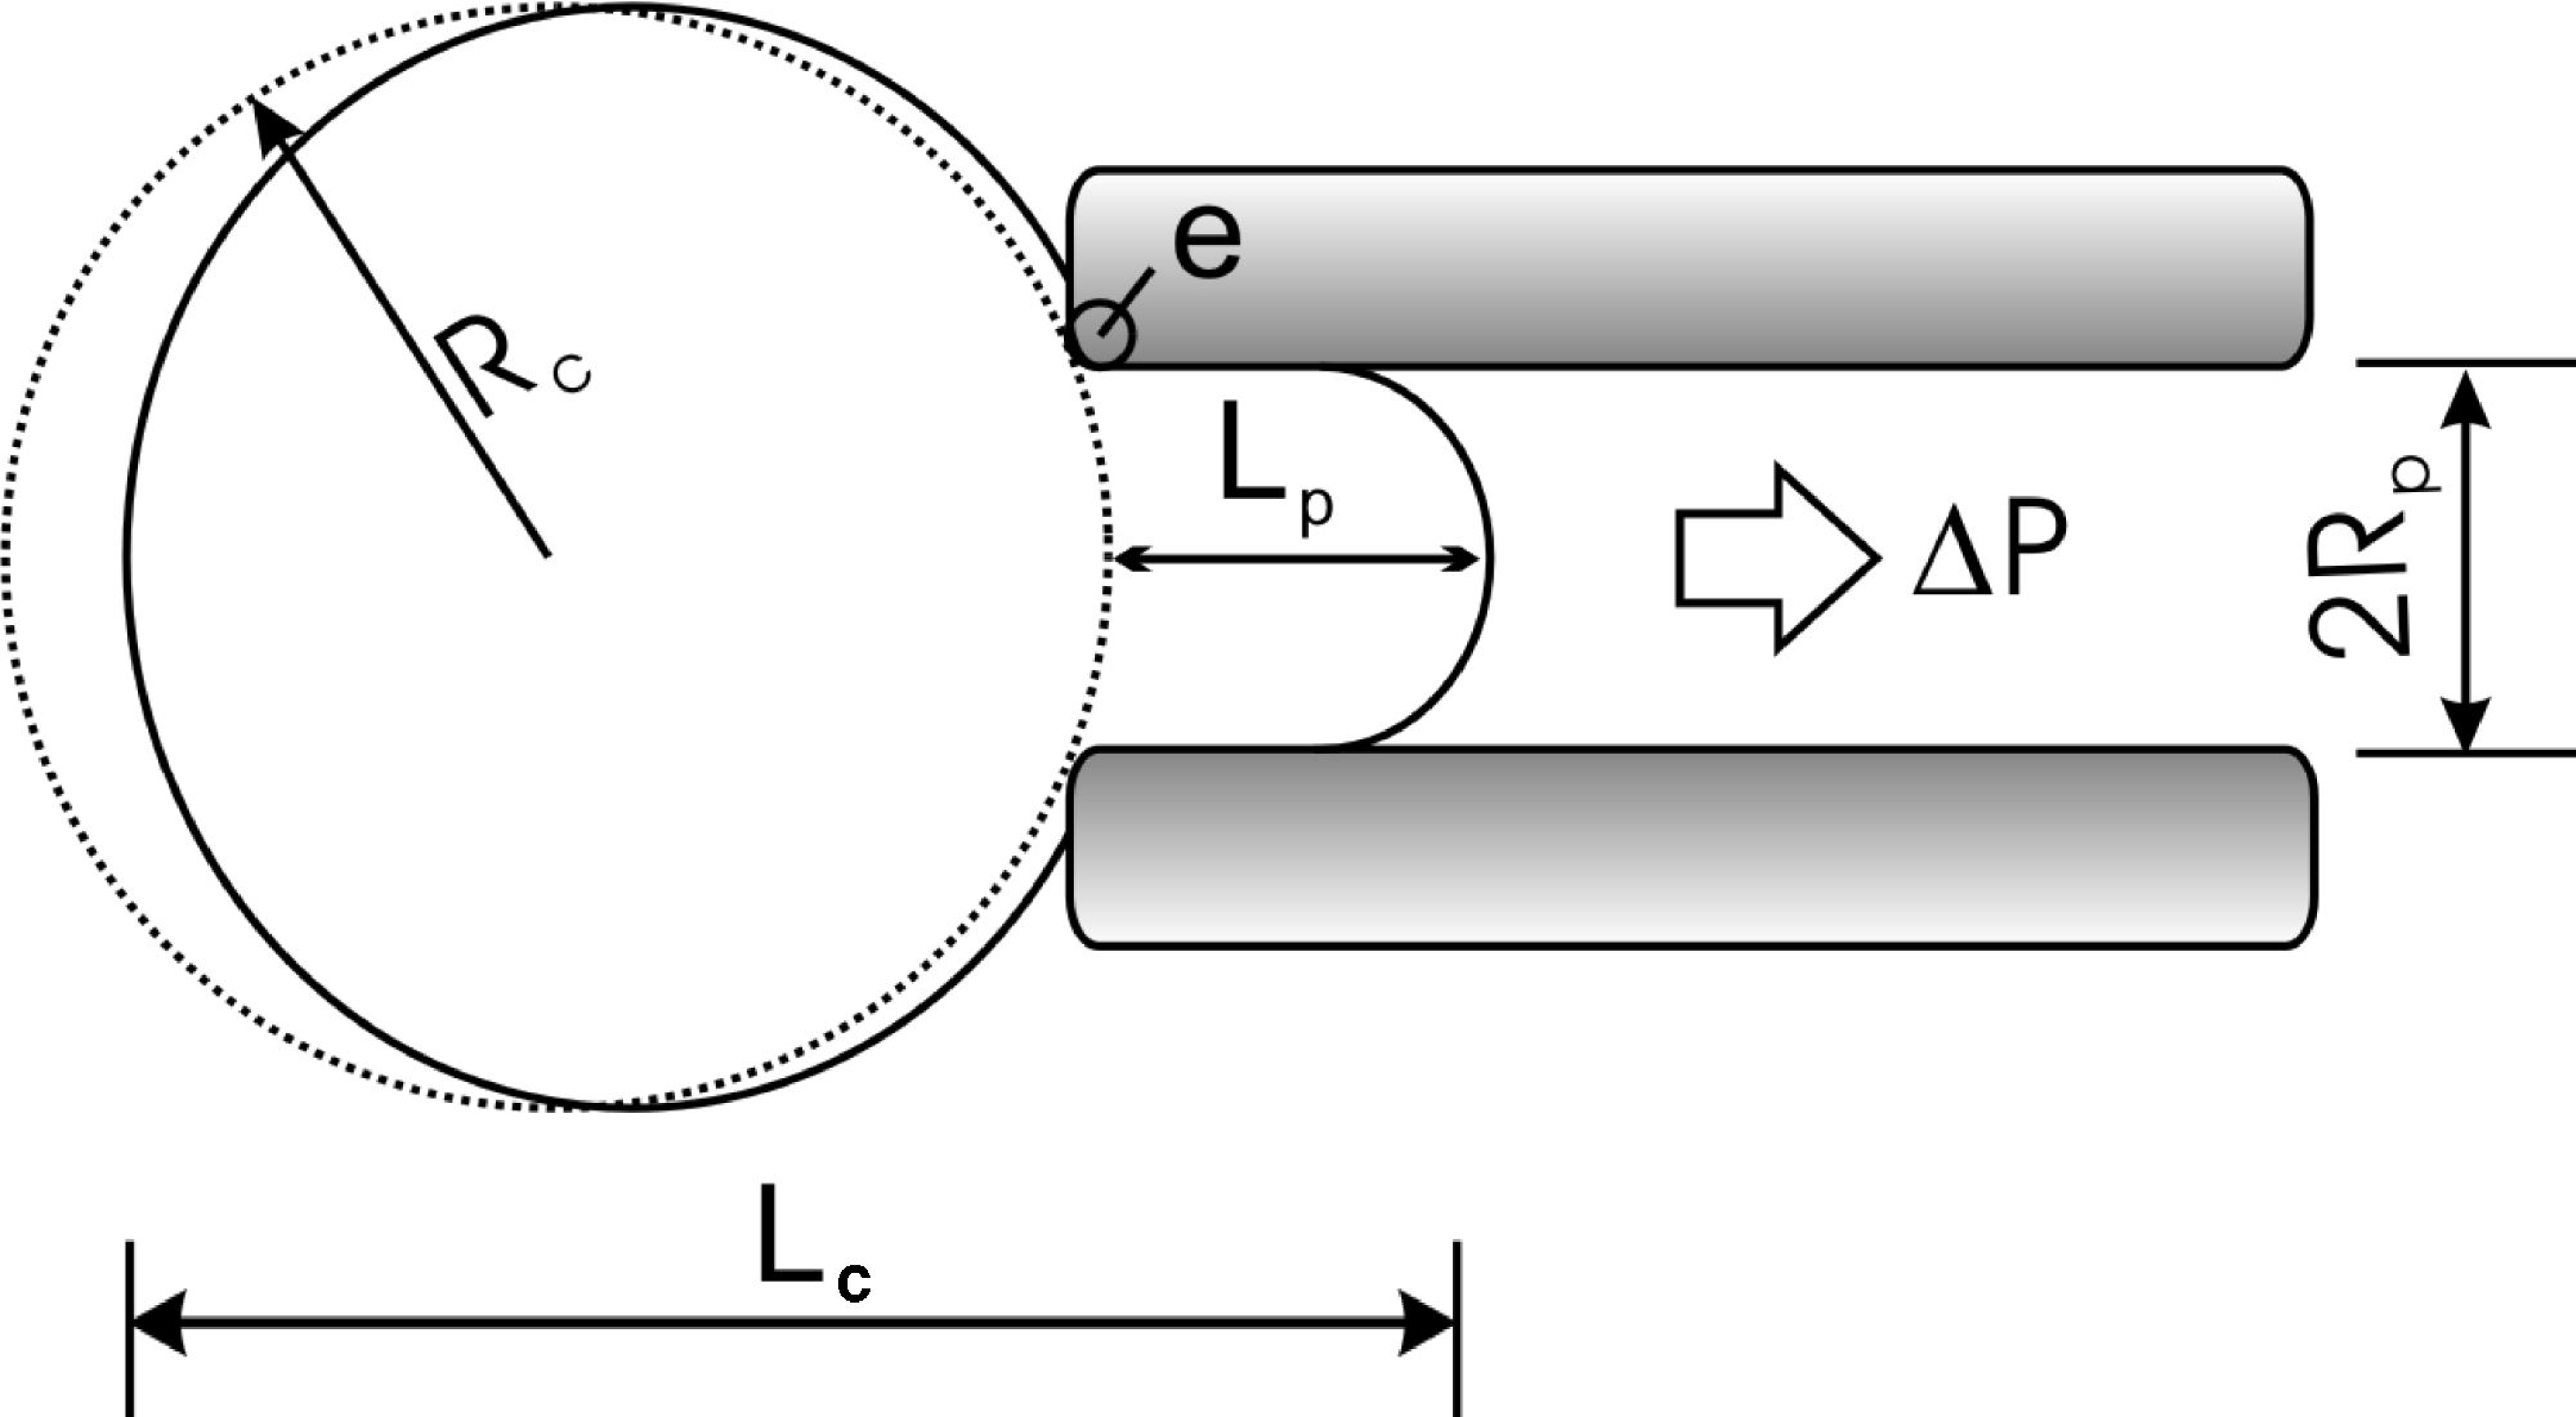
\includegraphics[width=\textwidth]{cellexp.pdf}
  \end{column}
  \begin{column}[b]{0.48\textwidth}
  \begin{itemize}
  \item 1964年, Rand和Burton首次应用微吸管测得人体红细胞膜的弹性模量.
  \item Evans和Hochmuth对细胞在微吸管实验中的变形恢复过程进行了研究.
  \end{itemize}
  \end{column}
\end{columns}
}
\subsection{细胞力学模型简介}
\frame{\frametitle{经典细胞力学模型}
\begin{columns}
  \begin{column}[b]{0.4\textwidth}
\begin{center}
 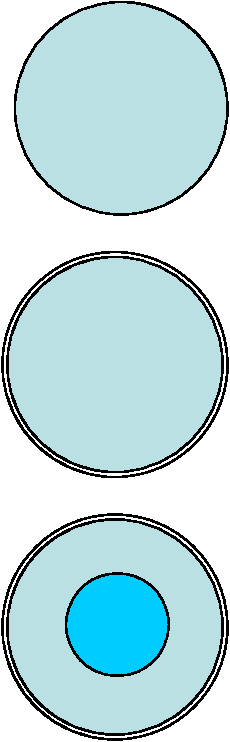
\includegraphics[width=0.3\textwidth]{model.pdf}
\end{center}
  \end{column}
  \begin{column}[b]{0.6\textwidth}
 \begin{itemize}
  \item 固体模型:细胞假设成均匀的且不含明显皮层的不可压缩弹性或者粘弹性固体.
  \item 液体模型:将细胞内部看成均匀同一的牛顿粘性流体, 细胞皮层具有张力.
  \item 复合液滴模型:在液体模型的基础上用一个封装的液滴来表示细胞核.
  \end{itemize}
  \end{column}
\end{columns}

}


